\documentclass{article}
\usepackage{amsthm}
\usepackage{amsmath}
\usepackage{graphicx}
\usepackage{color}
\usepackage{subfig}
\usepackage{physics}
\graphicspath{ {figures/} }

\begin{document}

We begin with looking at a $10\times 10$ system - that is, we have two layers of $100$ spins each. First,
we can look at the plot of the magnetization vs. external field $B$. Magnetization $M$ represents the normalized magnetization of the entire system, while $M_{1}$
and $M_{2}$ are the individual normalized magnetizations of each layer.


\begin{figure}

  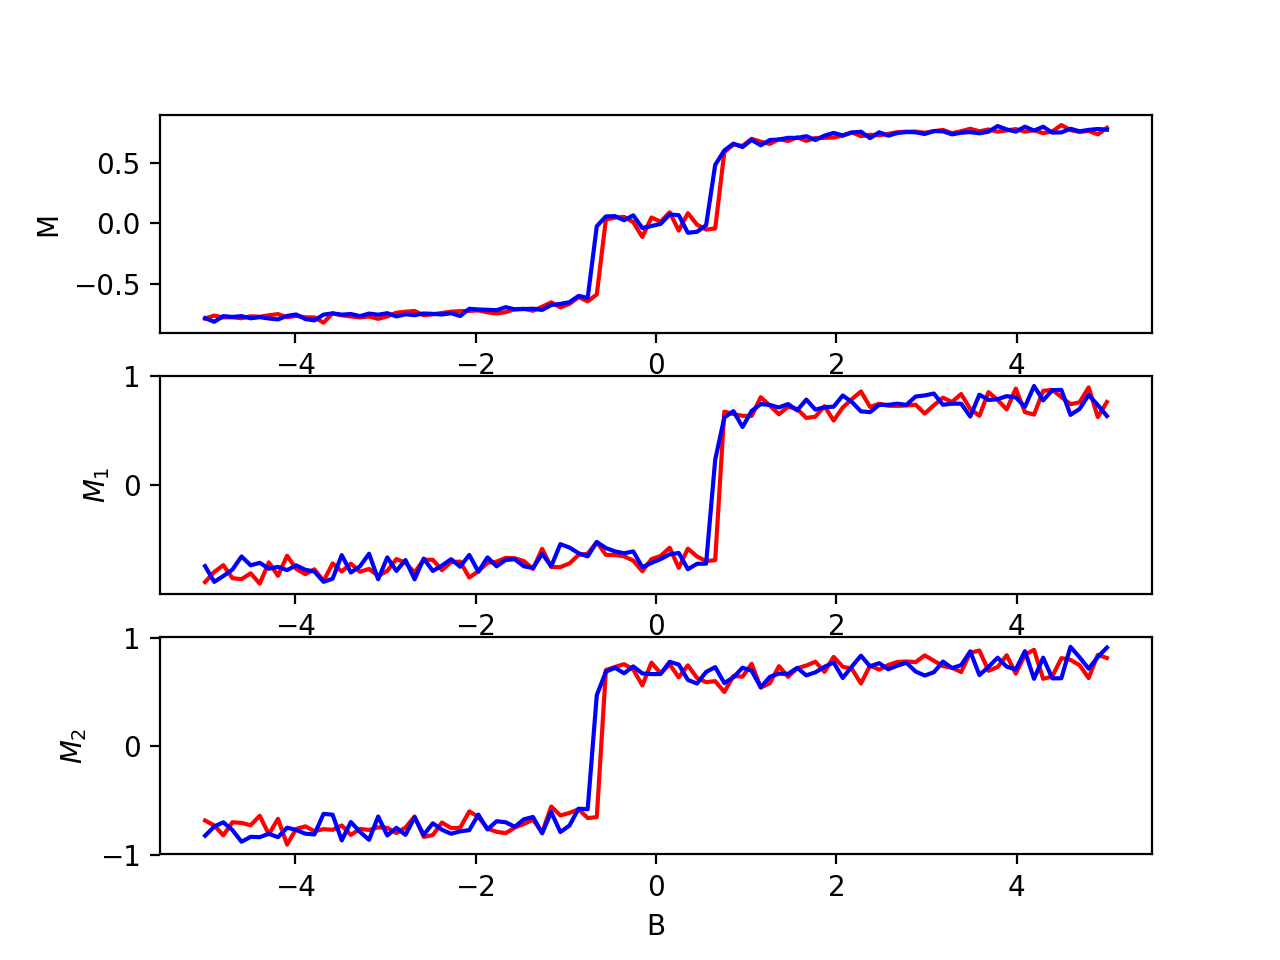
\includegraphics[width=\textwidth]{figures/magvb_anneal1.png}

\caption{Magnetization vs external field strength $B$ for $10 \times 10$ lattice at temperature $T = .5$. Anistropic
strength $k$ is set at $-1$ for both layers. Both interlayer and intralayer interactions strengths are set to $1$.}
\end{figure}

In the following plot, we see magnetization as a function of the anisotropic strength.


\begin{figure}

  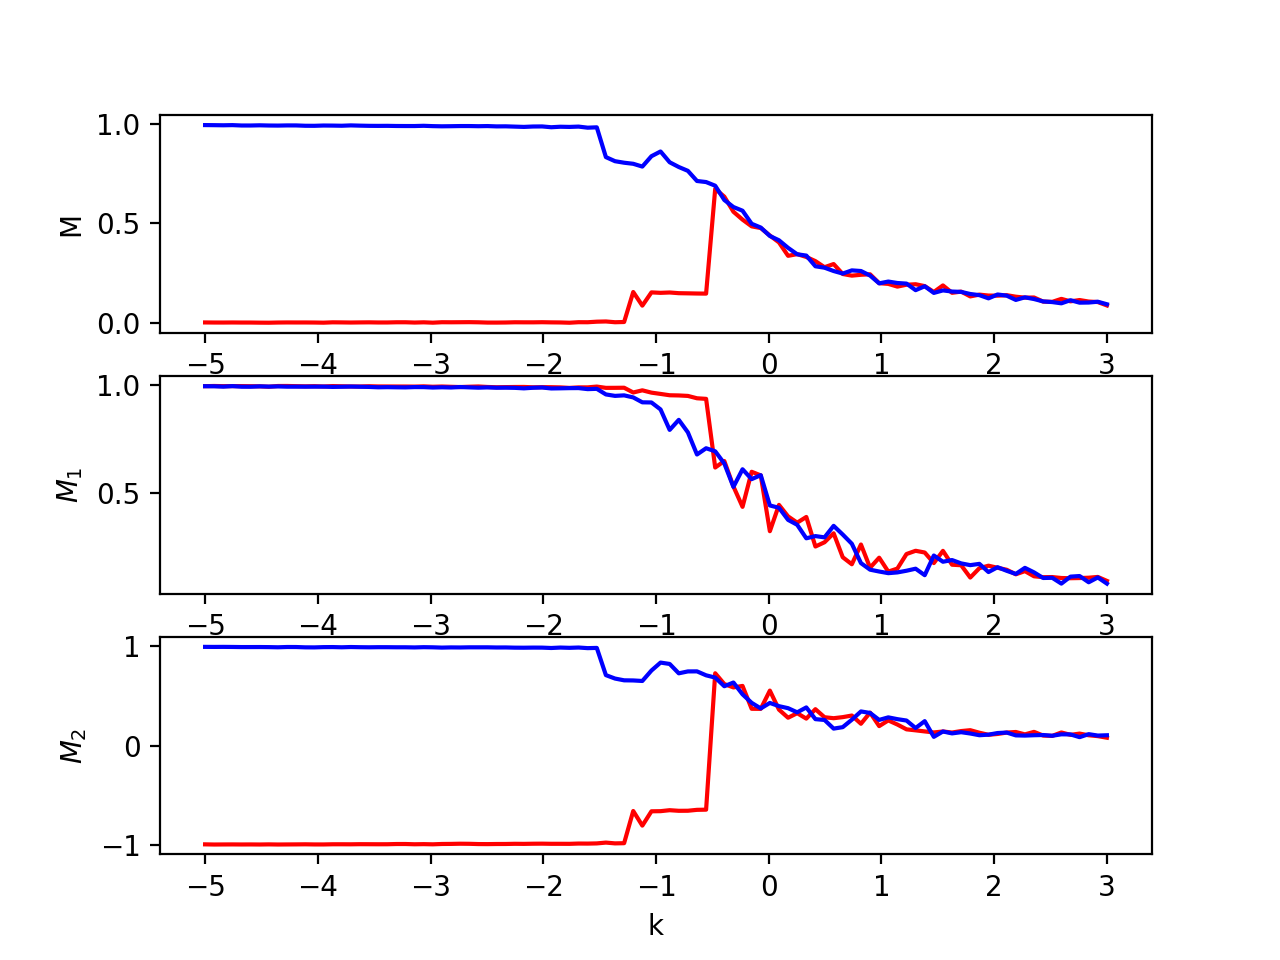
\includegraphics[width=\textwidth]{figures/magvk_1010_b.75_2.png}

\caption{Magnetization vs anisotropic strength $k$ for $10 \times 10$ lattice at temperature $T = .1$. Anistropic
strength $k$ ranges from $-5$ to $5$, with negative values indicating easy axis anisotropy. Both interlayer and intralayer interactions strengths are set to $1$.}
\end{figure}


\end{document}
